% Created by tikzDevice version 0.12.6 on 2026-08-03 03:41:24
% !TEX encoding = UTF-8 Unicode
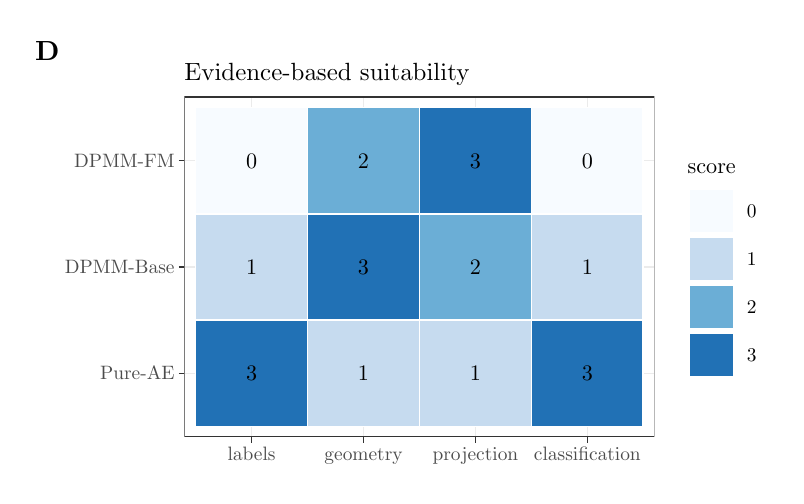
\begin{tikzpicture}[x=1pt,y=1pt]
\definecolor{fillColor}{RGB}{255,255,255}
\path[use as bounding box,fill=fillColor,fill opacity=0.00] (0,0) rectangle (270.41,161.83);
\begin{scope}
\path[clip] (  0.66,  1.74) rectangle (269.74,160.09);
\definecolor{drawColor}{RGB}{255,255,255}
\definecolor{fillColor}{RGB}{255,255,255}

\path[draw=drawColor,line width= 0.4pt,line join=round,line cap=round,fill=fillColor] (  0.66,  1.74) rectangle (269.74,160.09);
\end{scope}
\begin{scope}
\path[clip] ( 56.66, 13.93) rectangle (226.49,136.79);
\definecolor{fillColor}{RGB}{255,255,255}

\path[fill=fillColor] ( 56.66, 13.93) rectangle (226.49,136.79);
\definecolor{drawColor}{gray}{0.92}

\path[draw=drawColor,line width= 0.4pt,line join=round] ( 56.66, 36.97) --
	(226.49, 36.97);

\path[draw=drawColor,line width= 0.4pt,line join=round] ( 56.66, 75.36) --
	(226.49, 75.36);

\path[draw=drawColor,line width= 0.4pt,line join=round] ( 56.66,113.76) --
	(226.49,113.76);

\path[draw=drawColor,line width= 0.4pt,line join=round] ( 80.92, 13.93) --
	( 80.92,136.79);

\path[draw=drawColor,line width= 0.4pt,line join=round] (121.36, 13.93) --
	(121.36,136.79);

\path[draw=drawColor,line width= 0.4pt,line join=round] (161.79, 13.93) --
	(161.79,136.79);

\path[draw=drawColor,line width= 0.4pt,line join=round] (202.23, 13.93) --
	(202.23,136.79);
\definecolor{drawColor}{RGB}{255,255,255}
\definecolor{fillColor}{RGB}{33,113,181}

\path[draw=drawColor,line width= 0.6pt,fill=fillColor] ( 60.70, 17.77) rectangle (101.14, 56.17);
\definecolor{fillColor}{RGB}{198,219,239}

\path[draw=drawColor,line width= 0.6pt,fill=fillColor] ( 60.70, 56.17) rectangle (101.14, 94.56);
\definecolor{fillColor}{RGB}{247,251,255}

\path[draw=drawColor,line width= 0.6pt,fill=fillColor] ( 60.70, 94.56) rectangle (101.14,132.95);
\definecolor{fillColor}{RGB}{198,219,239}

\path[draw=drawColor,line width= 0.6pt,fill=fillColor] (101.14, 17.77) rectangle (141.58, 56.17);
\definecolor{fillColor}{RGB}{33,113,181}

\path[draw=drawColor,line width= 0.6pt,fill=fillColor] (101.14, 56.17) rectangle (141.58, 94.56);
\definecolor{fillColor}{RGB}{107,174,214}

\path[draw=drawColor,line width= 0.6pt,fill=fillColor] (101.14, 94.56) rectangle (141.58,132.95);
\definecolor{fillColor}{RGB}{198,219,239}

\path[draw=drawColor,line width= 0.6pt,fill=fillColor] (141.58, 17.77) rectangle (182.01, 56.17);
\definecolor{fillColor}{RGB}{107,174,214}

\path[draw=drawColor,line width= 0.6pt,fill=fillColor] (141.58, 56.17) rectangle (182.01, 94.56);
\definecolor{fillColor}{RGB}{33,113,181}

\path[draw=drawColor,line width= 0.6pt,fill=fillColor] (141.58, 94.56) rectangle (182.01,132.95);

\path[draw=drawColor,line width= 0.6pt,fill=fillColor] (182.01, 17.77) rectangle (222.45, 56.17);
\definecolor{fillColor}{RGB}{198,219,239}

\path[draw=drawColor,line width= 0.6pt,fill=fillColor] (182.01, 56.17) rectangle (222.45, 94.56);
\definecolor{fillColor}{RGB}{247,251,255}

\path[draw=drawColor,line width= 0.6pt,fill=fillColor] (182.01, 94.56) rectangle (222.45,132.95);
\definecolor{drawColor}{RGB}{0,0,0}

\node[text=drawColor,anchor=base,inner sep=0pt, outer sep=0pt, scale=  0.80] at ( 80.92, 34.23) {3};

\node[text=drawColor,anchor=base,inner sep=0pt, outer sep=0pt, scale=  0.80] at ( 80.92, 72.62) {1};

\node[text=drawColor,anchor=base,inner sep=0pt, outer sep=0pt, scale=  0.80] at ( 80.92,111.01) {0};

\node[text=drawColor,anchor=base,inner sep=0pt, outer sep=0pt, scale=  0.80] at (121.36, 34.23) {1};

\node[text=drawColor,anchor=base,inner sep=0pt, outer sep=0pt, scale=  0.80] at (121.36, 72.62) {3};

\node[text=drawColor,anchor=base,inner sep=0pt, outer sep=0pt, scale=  0.80] at (121.36,111.01) {2};

\node[text=drawColor,anchor=base,inner sep=0pt, outer sep=0pt, scale=  0.80] at (161.79, 34.23) {1};

\node[text=drawColor,anchor=base,inner sep=0pt, outer sep=0pt, scale=  0.80] at (161.79, 72.62) {2};

\node[text=drawColor,anchor=base,inner sep=0pt, outer sep=0pt, scale=  0.80] at (161.79,111.01) {3};

\node[text=drawColor,anchor=base,inner sep=0pt, outer sep=0pt, scale=  0.80] at (202.23, 34.23) {3};

\node[text=drawColor,anchor=base,inner sep=0pt, outer sep=0pt, scale=  0.80] at (202.23, 72.62) {1};

\node[text=drawColor,anchor=base,inner sep=0pt, outer sep=0pt, scale=  0.80] at (202.23,111.01) {0};
\definecolor{drawColor}{gray}{0.20}

\path[draw=drawColor,line width= 0.4pt,line join=round,line cap=round] ( 56.66, 13.93) rectangle (226.49,136.79);
\end{scope}
\begin{scope}
\path[clip] (  0.00,  0.00) rectangle (270.41,161.83);
\definecolor{drawColor}{gray}{0.30}

\node[text=drawColor,anchor=base east,inner sep=0pt, outer sep=0pt, scale=  0.70] at ( 53.06, 34.56) {Pure-AE};

\node[text=drawColor,anchor=base east,inner sep=0pt, outer sep=0pt, scale=  0.70] at ( 53.06, 72.95) {DPMM-Base};

\node[text=drawColor,anchor=base east,inner sep=0pt, outer sep=0pt, scale=  0.70] at ( 53.06,111.35) {DPMM-FM};
\end{scope}
\begin{scope}
\path[clip] (  0.00,  0.00) rectangle (270.41,161.83);
\definecolor{drawColor}{gray}{0.20}

\path[draw=drawColor,line width= 0.4pt,line join=round] ( 54.66, 36.97) --
	( 56.66, 36.97);

\path[draw=drawColor,line width= 0.4pt,line join=round] ( 54.66, 75.36) --
	( 56.66, 75.36);

\path[draw=drawColor,line width= 0.4pt,line join=round] ( 54.66,113.76) --
	( 56.66,113.76);
\end{scope}
\begin{scope}
\path[clip] (  0.00,  0.00) rectangle (270.41,161.83);
\definecolor{drawColor}{gray}{0.20}

\path[draw=drawColor,line width= 0.4pt,line join=round] ( 80.92, 11.93) --
	( 80.92, 13.93);

\path[draw=drawColor,line width= 0.4pt,line join=round] (121.36, 11.93) --
	(121.36, 13.93);

\path[draw=drawColor,line width= 0.4pt,line join=round] (161.79, 11.93) --
	(161.79, 13.93);

\path[draw=drawColor,line width= 0.4pt,line join=round] (202.23, 11.93) --
	(202.23, 13.93);
\end{scope}
\begin{scope}
\path[clip] (  0.00,  0.00) rectangle (270.41,161.83);
\definecolor{drawColor}{gray}{0.30}

\node[text=drawColor,anchor=base,inner sep=0pt, outer sep=0pt, scale=  0.70] at ( 80.92,  5.51) {labels};

\node[text=drawColor,anchor=base,inner sep=0pt, outer sep=0pt, scale=  0.70] at (121.36,  5.51) {geometry};

\node[text=drawColor,anchor=base,inner sep=0pt, outer sep=0pt, scale=  0.70] at (161.79,  5.51) {projection};

\node[text=drawColor,anchor=base,inner sep=0pt, outer sep=0pt, scale=  0.70] at (202.23,  5.51) {classification};
\end{scope}
\begin{scope}
\path[clip] (  0.00,  0.00) rectangle (270.41,161.83);
\definecolor{fillColor}{RGB}{255,255,255}

\path[fill=fillColor] (234.49, 30.91) rectangle (267.74,119.82);
\end{scope}
\begin{scope}
\path[clip] (  0.00,  0.00) rectangle (270.41,161.83);
\definecolor{drawColor}{RGB}{0,0,0}

\node[text=drawColor,anchor=base west,inner sep=0pt, outer sep=0pt, scale=  0.80] at (238.49,109.30) {score};
\end{scope}
\begin{scope}
\path[clip] (  0.00,  0.00) rectangle (270.41,161.83);
\definecolor{fillColor}{RGB}{255,255,255}

\path[fill=fillColor] (238.49, 86.94) rectangle (255.84,104.29);
\definecolor{drawColor}{RGB}{255,255,255}
\definecolor{fillColor}{RGB}{247,251,255}

\path[draw=drawColor,line width= 0.6pt,fill=fillColor] (239.20, 87.65) rectangle (255.13,103.57);
\end{scope}
\begin{scope}
\path[clip] (  0.00,  0.00) rectangle (270.41,161.83);
\definecolor{fillColor}{RGB}{255,255,255}

\path[fill=fillColor] (238.49, 69.60) rectangle (255.84, 86.94);
\definecolor{drawColor}{RGB}{255,255,255}
\definecolor{fillColor}{RGB}{198,219,239}

\path[draw=drawColor,line width= 0.6pt,fill=fillColor] (239.20, 70.31) rectangle (255.13, 86.23);
\end{scope}
\begin{scope}
\path[clip] (  0.00,  0.00) rectangle (270.41,161.83);
\definecolor{fillColor}{RGB}{255,255,255}

\path[fill=fillColor] (238.49, 52.25) rectangle (255.84, 69.60);
\definecolor{drawColor}{RGB}{255,255,255}
\definecolor{fillColor}{RGB}{107,174,214}

\path[draw=drawColor,line width= 0.6pt,fill=fillColor] (239.20, 52.96) rectangle (255.13, 68.88);
\end{scope}
\begin{scope}
\path[clip] (  0.00,  0.00) rectangle (270.41,161.83);
\definecolor{fillColor}{RGB}{255,255,255}

\path[fill=fillColor] (238.49, 34.91) rectangle (255.84, 52.25);
\definecolor{drawColor}{RGB}{255,255,255}
\definecolor{fillColor}{RGB}{33,113,181}

\path[draw=drawColor,line width= 0.6pt,fill=fillColor] (239.20, 35.62) rectangle (255.13, 51.54);
\end{scope}
\begin{scope}
\path[clip] (  0.00,  0.00) rectangle (270.41,161.83);
\definecolor{drawColor}{RGB}{0,0,0}

\node[text=drawColor,anchor=base west,inner sep=0pt, outer sep=0pt, scale=  0.70] at (259.84, 93.20) {0};
\end{scope}
\begin{scope}
\path[clip] (  0.00,  0.00) rectangle (270.41,161.83);
\definecolor{drawColor}{RGB}{0,0,0}

\node[text=drawColor,anchor=base west,inner sep=0pt, outer sep=0pt, scale=  0.70] at (259.84, 75.86) {1};
\end{scope}
\begin{scope}
\path[clip] (  0.00,  0.00) rectangle (270.41,161.83);
\definecolor{drawColor}{RGB}{0,0,0}

\node[text=drawColor,anchor=base west,inner sep=0pt, outer sep=0pt, scale=  0.70] at (259.84, 58.51) {2};
\end{scope}
\begin{scope}
\path[clip] (  0.00,  0.00) rectangle (270.41,161.83);
\definecolor{drawColor}{RGB}{0,0,0}

\node[text=drawColor,anchor=base west,inner sep=0pt, outer sep=0pt, scale=  0.70] at (259.84, 41.17) {3};
\end{scope}
\begin{scope}
\path[clip] (  0.00,  0.00) rectangle (270.41,161.83);
\definecolor{drawColor}{RGB}{0,0,0}

\node[text=drawColor,anchor=base west,inner sep=0pt, outer sep=0pt, scale=  0.90] at ( 56.66,142.78) {Evidence-based suitability};
\end{scope}
\begin{scope}
\path[clip] (  0.00,  0.00) rectangle (270.41,161.83);
\definecolor{drawColor}{RGB}{0,0,0}

\node[text=drawColor,anchor=base,inner sep=0pt, outer sep=0pt, scale=  1.00] at (  7.07,150.08) {\bfseries D};
\end{scope}
\end{tikzpicture}
